\section{Unit Step Signal}
The unit step signal, also known as the Heaviside step function, is
0 for values less than 0 and 1 otherwise. 

\subsection{Discrete-Time Unit Step Signal}
The discrete-time unit step signal is defined as:
\[
u[n] =
\begin{cases}
1 & n \geq 0, \\
0 & n < 0.
\end{cases}
\]

Below is the plot for the discrete-time unit step signal:
\[
u[n] = 1 \text{ for } n \geq 0, \text{ and } u[n] = 0 \text{ for } n < 0.
\]

\begin{figure}[h!]
\centering
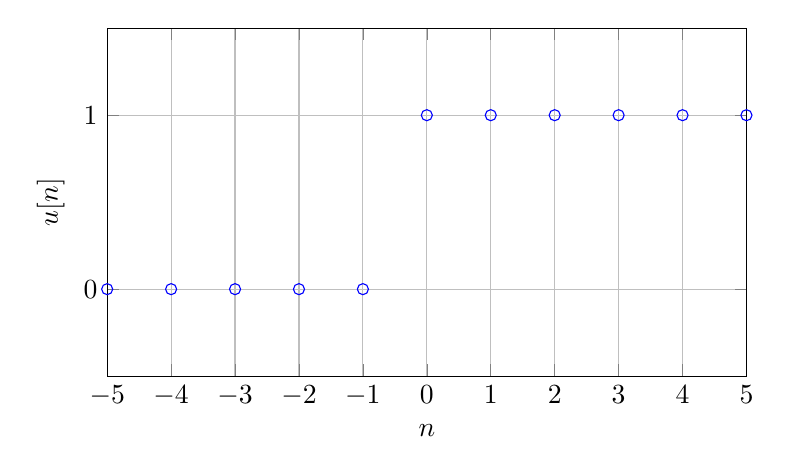
\begin{tikzpicture}
    \begin{axis}[
        xlabel={$n$},
        ylabel={$u[n]$},
        grid=major,
        ytick={0,1},
        xtick={-5,-4,...,5},
        ymin=-0.5, ymax=1.5,
        xmin=-5, xmax=5,
        width=0.8\textwidth,
        height=6cm,
        samples=100,
        domain=-5:5
    ]
    \addplot+[only marks, mark=o] coordinates {
        (-5,0) (-4,0) (-3,0) (-2,0) (-1,0)
        (0,1) (1,1) (2,1) (3,1) (4,1) (5,1)
    };
    \end{axis}
\end{tikzpicture}
\caption{Discrete-Time Unit Step Signal}
\end{figure}

\subsection{Continuous-Time Unit Step Signal}
The continuous-time unit step signal is defined as:
\[
u(t) =
\begin{cases}
1 & t \geq 0, \\
0 & t < 0.
\end{cases}
\]

Below is the plot for the continuous-time unit step signal:

\begin{figure}[h!]
\centering
\begin{tikzpicture}
    \begin{axis}[
        xlabel={$t$},
        ylabel={$u(t)$},
        grid=major,
        ytick={0,1},
        xmin=-5, xmax=5,
        ymin=-0.5, ymax=1.5,
        width=0.8\textwidth,
        height=6cm,
        samples=100,
        domain=-5:5
    ]
    \addplot[domain=-5:0, samples=100, thick] {0};
    \addplot[domain=0:5, samples=100, thick] {1};
    \addplot[mark=*, mark size=2pt] coordinates {(0,1)};
    \end{axis}
\end{tikzpicture}
\caption{Continuous-Time Unit Step Signal}
\end{figure}

